\chapter{Impulse, Torque and Angular Momentum for a system of particles}

\section{Linear Impulse and Momentum}

Newtons second law for a single particle can be expressed as:
\begin{equation}
	F_{ext} = m a = m \frac{d}{dt}v
\end{equation}
for a system of particles,
\begin{equation}
\sum F_{ext} = m a = m \frac{d}{dt}v
\end{equation}
Linear impulse is a accumulation of forces acting on each of the particle, this can be found using integral:
\begin{equation}
\int_{t_{1}}^{t_{2}} \sum F_{ext} dt = \int_{v_{1}}^{v_{2}} m dv
\end{equation}
simplifying the above equation:
\begin{equation}
 \sum \int_{t_{1}}^{t_{2}} F_{ext} dt = m v_{2} - m v_{1}
\end{equation}
or in a standard form, this can be expressed as
\begin{equation}\label{Eq_0_ch2_ImpulseMometumEquation}
m v_{1} + \sum \int_{t_{1}}^{t_{2}} F_{ext} dt = m v_{2}
\end{equation}

\subsection{Problem on Impulse - Momentum}

Consider figure \ref{fig_0_ch_0_ImpulseMomentumProblem}. 
\newpage
\begin{figure}[h!]
	\centering
	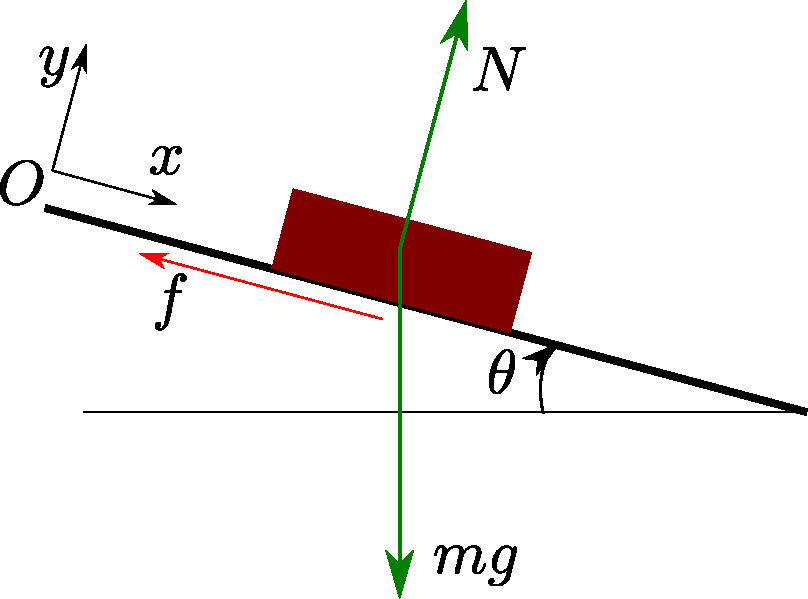
\includegraphics[width=0.6\linewidth]{Bilder/09_ImpulseProblem.pdf}
	\caption{Impulse - Momentum Problem}
	\label{fig_0_ch_0_ImpulseMomentumProblem}
\end{figure}
summation on the external forces leads to
\begin{equation} \label{Eq_0_ch_2_ImpulseMomentumProblemEq1}
	\sum F_{x} = (mg sin\theta - \mu mg cos\theta) = k
\end{equation}
Let initial velocity $v_{x1} = 0$ at time $t = 0$. equation \eqref{Eq_0_ch_2_ImpulseMomentumProblemEq1} is a constant in time, therefore it can be expressed using a single constant character $k$. Using impulse-momentum equation given by equation \eqref{Eq_0_ch2_ImpulseMometumEquation} and substituting for $\sum F_{ext}$, we get:
\begin{equation}
	\int_{0}^{t} k dt = m v_{2x} \implies k t \Big|_0^t = m v_{2x} \implies v_{2x} = \frac{k t}{m}
\end{equation}

\section{Momentum for system of particles}

For a system of particles, with $i$ number of particles, the center of mass of all the system of particles can be expressed by $m_{T}$. Using the center of mass definition, the momentum of all the particles can be expressed as:
\begin{equation}
	m_{T} v_{G/O} = \sum _i m_{i} v_{i/O}
\end{equation}
taking time-derivative:
\begin{equation}
m_{T} \dot{v}_{G/O} = \sum _i m_{i} \frac{d}{dt} v_{i/O} \implies m_{T} \dot{v}_{G/O} = \sum F_{i_{ext}}
\end{equation}
to determine impulse, taking the time integral on both sides of the equation:
\begin{equation} \label{Eq_0_ch_2_MomentumEquationForSystemOfParticles}
	\int_{t_{1}}^{t_{2}} \sum F_{i_{ext}} = int_{t_{1}}^{t_{2}} m_{T} \frac{d}{dt}{v}_{G/O} \implies \int_{t_{1}}^{t_{2}} \sum F_{i_{ext}} dt = m_{T} \left[ {v}_{G/O} \Big |_1 - {v}_{G/O} \Big |_2 \right] 
\end{equation}

\subsection{Problem on momentum on system of particles}

Consider figure \ref{fig_0_ch_2_MomentumProblemOnSystemOfParticles}.
\begin{figure}[h!]
	\centering
	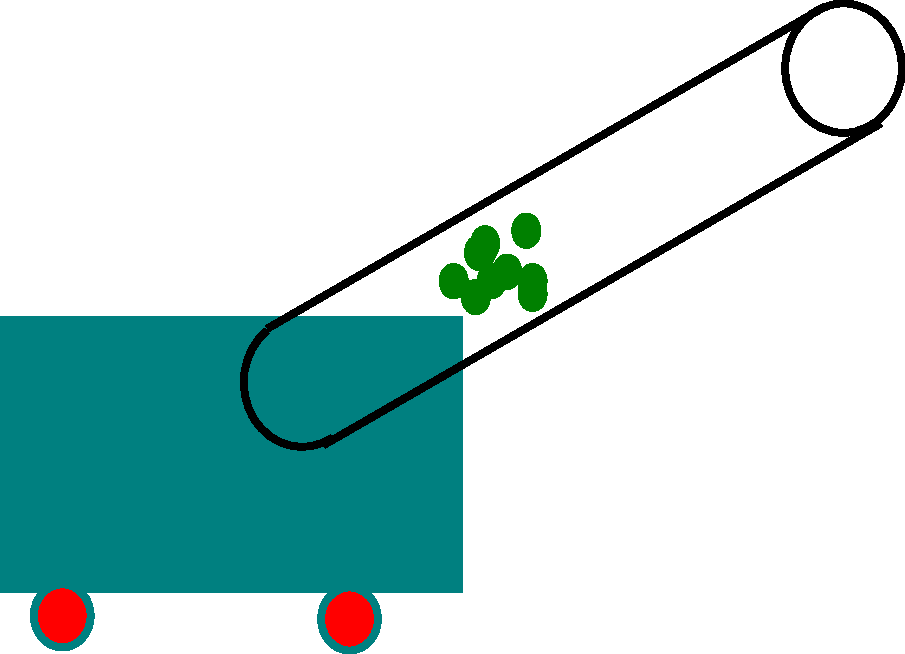
\includegraphics[width=0.5\linewidth]{Bilder/10_MometumSystemOfParticles.pdf}
	\caption{Momentum problem on system of particles}
	\label{fig_0_ch_2_MomentumProblemOnSystemOfParticles}
\end{figure}

For the system of particles (green) inside the canon, the reaction force acting on the canon due to an explosive denoting the particles can be determined using the momentum equation for the system of particles given by equation \eqref{Eq_0_ch_2_MomentumEquationForSystemOfParticles}. 

Let the total mass of the shot (system of particles) is $10 kg$, length of the barrel $7 m$ and the exit velocity of the shot $215 m/s$.

As the shot was idle initially, the initial velocity is $v_{0} = 0 m/s$, final velocity $v_{f} = 215 m/s$, we can find average velocity as
\begin{equation}
	v_{avg} = (v_{f} - v_{0}) / 2 \implies v_{avg} = 107.5 m/s
\end{equation}
further average velocity is also:
\begin{equation}
	v_{avg} = \frac{distance}{\Delta t} \implies \Delta t = \frac{7 m}{107.5 m/s} = 0.065s
\end{equation}
using the momentum equation \eqref{Eq_0_ch_2_MomentumEquationForSystemOfParticles}:
\begin{equation}
	\int_{t_{1}}^{t_{2}} \sum F_{i_{ext}} dt = \frac{10 kg}{9.81 m/s^{2}} \left( 215 m/s \right) \implies F_{i_{ext}} \Delta t = \frac{10 kg}{9.81 m/s^{2}} \left( 215 m/s \right)
\end{equation}
which simplifies to:
\begin{equation}
	F_{i_{ext}} = \frac{10 kg}{9.81 m/s^{2} * \Delta t} \left( 215 m/s \right) = 3.65 kN
\end{equation}

\section{Angular Momentum of a particle}

Angular momentum is defined as the moment of the momentum. Consider figure \ref{fig_0_ch_0_anugularMomentumwrtO}, let particle B subjected to forces $f_{B}$, B is also translating so it has a momentum given by $p_{B/O}$. \textbf{\textit{Note: }}Linear momentum is always expressed w.r.t the inertial frame. 
\begin{figure}[h!]
	\centering
	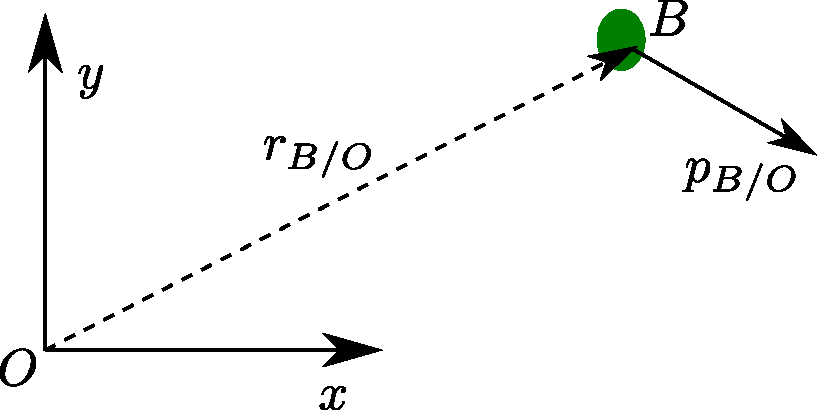
\includegraphics[width=0.6\linewidth]{Bilder/11_AnularMomentumParticle.pdf}
	\caption{Angular momentum of B w.r.t O}
	\label{fig_0_ch_0_anugularMomentumwrtO}
\end{figure}
From the definition of angular momentum,
\begin{equation} \label{eq_0_ch_2_angualrMomentumofAParticle}
	h_{B/O} = r_{B/O} \times p_{B/O}
\end{equation}
torque is defined as the rate of change angular momentum as net total of all the external torques acting on the system,
\begin{equation}
	\frac{d}{dt}(h_{B/O}) = \sum \tau_{B/O}
\end{equation}
\begin{figure}[h!]
	\centering
	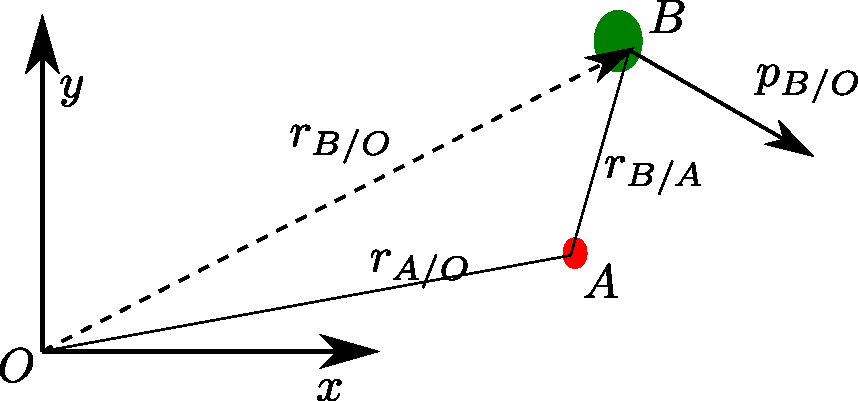
\includegraphics[width=0.6\linewidth]{Bilder/12_AnularMomentumParticle.pdf}
	\caption{Angular momentum of B w.r.t A}
	\label{fig_0_ch_0_anugularMomentumwrtB}
\end{figure}
Lets consider an arbitrary point A, if we compute angular momentum of B w.r.t A as shown in figure \ref{fig_0_ch_0_anugularMomentumwrtB}, the linear momentum is always w.r.t the inertial frame
\begin{equation}
	h_{B/A} = r_{B/A} \times p_{B/O}
\end{equation}
torque required for this system in order to change the angular momentum can be determined as follows:

Let the arm length between A and B be fixed (like in Robotics) such that there is no translation between B and A. In this case, the time derivative can be calculated as follows:
\begin{equation} \label{Eq_0_ch_0_TorqueOfAprticleEq1}
	\sum \tau_{B/A} = \frac{d}{dt} (r_{B/A} \times p_{B/O}) = r_{B/A} \times \frac{d}{dt} p_{B/O}
\end{equation}

Note that equation \eqref{Eq_0_ch_0_TorqueOfAprticleEq1} is of the following form
\begin{equation}\label{eq_0_ch_0_TorqueOfAprticleEq12}
	\sum \tau_{B/A} = r_{B/A} \times f_{B} = r_{B/A} \times \frac{d}{dt} p_{B/O} = Q
\end{equation}
in this case, the net effect of all the forces acting at B results in change in momentum i.e. $p_{B/O}$. Further from mathematics, $Q$ is of the form:
\begin{equation}\label{eq_0_ch_0_Qform}
	Q = a \times \frac{d}{dt}b = \frac{d}{dt}(a \times b) - \frac{d}{dt}a \times b
\end{equation}
using equation \eqref{eq_0_ch_0_Qform}, equation \eqref{eq_0_ch_0_TorqueOfAprticleEq12} can be expressed as
\begin{equation}\label{eq_0_ch_0_TorqueOfAprticleEq13}
	\sum \tau_{B/A} = \frac{d}{dt}(r_{B/A} \times p_{B/O}) - \frac{d}{dt}r_{B/A} \times p_{B/O}
\end{equation}
the terms of equation \eqref{eq_0_ch_0_TorqueOfAprticleEq12} are solved as follows
\begin{equation} \label{eq_0_ch_0_TorqueOfAprticleEq3}
	\frac{d}{dt}(r_{B/A} \times p_{B/O}) = \frac{d}{dt}(h_{B/A})
\end{equation}
\begin{equation}\label{eq_0_ch_0_TorqueOfAprticleEq4}
	r_{B/A} = r_{B/O} - r_{A/O} \implies v_{B/A} = v_{B/O} - v_{A/O}
\end{equation}
using equations (\eqref{eq_0_ch_0_TorqueOfAprticleEq3} and \eqref{eq_0_ch_0_TorqueOfAprticleEq4}) and substituting in equation \eqref{eq_0_ch_0_TorqueOfAprticleEq12}, we get the following
\begin{equation} \label{eq_0_ch_0_TorqueOfAprticleEq5}
	\sum \tau_{B/A} = \frac{d}{dt} h_{B/A} - \frac{d}{dt} (v_{B/O} - v_{A/O}) \times p_{B/O}
\end{equation}
further, in equation \eqref{eq_0_ch_0_TorqueOfAprticleEq5}, both $v_{B/O}$ and $p_{B/O}$ are pointing in the same direction as the linear momentum is always pointing the same direction as the linear velocity, the cross product of these will result in a zero, leaving behind only the cross product $v_{A/O} \times p_{B/O}$ as follows
\begin{equation}\label{eq_0_ch_0_TorqueOfAprticleEq6}
	\sum \tau_{B/A} = \frac{d}{dt} h_{B/A} + \frac{d}{dt} v_{A/O} \times p_{B/O}
\end{equation}
equation \eqref{eq_0_ch_0_TorqueOfAprticleEq6} is the expressing relating the net effect of torques and change in angular momentum at B w.r.t to an arbitrary point A. Equation \eqref{eq_0_ch_0_TorqueOfAprticleEq6} can now be further simplifies based on the application on the following cases:
\begin{itemize}
	\item case 1: when $v_{A/O} = 0$, i.e, point A is always fixed
	\item case 2: when $v_{A/O}$ and $p_{B/O}$ are parallel, happens in cases when $A$ is actually the center of mass for either the system of particles or for that of a rigid body
\end{itemize}
In both such cases, equation \eqref{eq_0_ch_0_TorqueOfAprticleEq6} reduces to
\begin{equation}\label{eq_0_ch_0_TorqueOfAprticleEq7}
\sum \tau_{B/A} = \frac{d}{dt} h_{B/A}
\end{equation}
equation \eqref{eq_0_ch_0_TorqueOfAprticleEq7} is the most simplified form of torque and angular momentum relationships, this form is most used for problems related to motion of wheels in robotics and automotive applications.

\subsection{Angular momentum and torque problem for a particle}

Consider figure \ref{fig_0_ch_0_angularMomentumProb}, where B is a ride which can go round and round with angular velocity $\omega = \dot{\theta}$ as well as translate with velocity $\dot{r}$, let both these velocities are constant. In this problem, as there are both the velocity terms $\dot{\theta}$ and $\dot{r}$, B experiences both the centripetal accelerations due to term $r\dot{\theta}^{2}$ and Coriolis acceleration due to the term $\dot{r}\dot{\theta}$. Further, as angular momentum is expressed as $r_{B/O} \times p_{B/O}$, as $r$ is changing, the angular momentum is changing. Additionally, as $v_{B/O}$ is changing due to $\dot{r}$, whenever, $dot{r}$ changes direction, linear momentum also changes direction, therefore, $p_{B/O}$ is also changing.
\begin{figure}[h!]
	\centering
	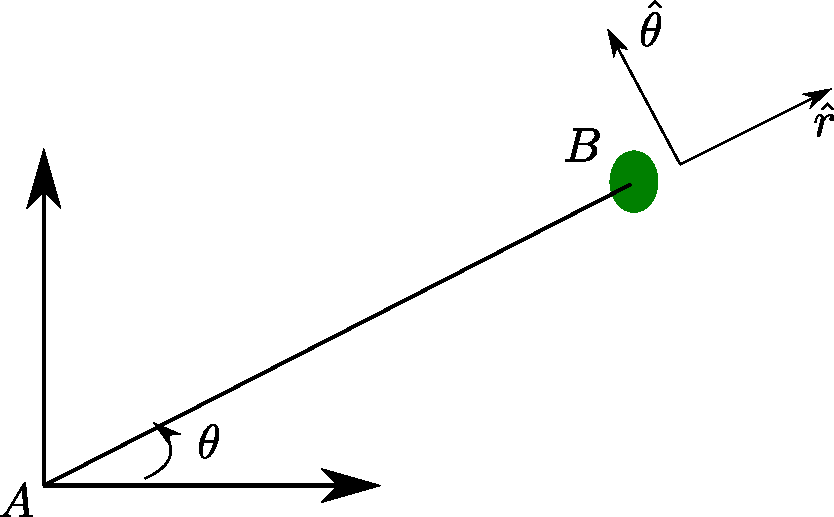
\includegraphics[width=0.6\linewidth]{Bilder/13_AngularMomentumProblem1.pdf}
	\caption{Angular momentum problem}
	\label{fig_0_ch_0_angularMomentumProb}
\end{figure}

\subsubsection{Angular momentum}
velocity of the particle B is expressed as
\begin{equation}
	v_{B/O} = \dot{r}\hat{r} + r \dot{\theta} \hat{\theta}
\end{equation}
angular momentum is expressed using equation \eqref{eq_0_ch_2_angualrMomentumofAParticle}:
\begin{equation}
	h_{B/A} = r_{B/A} \times p_{B/O} = r \hat{r} \times m \left( \dot{r}\hat{r} + r \dot{\theta} \hat{\theta} \right)
\end{equation}
simplifying the above equation we get:
\begin{equation}
	h_{B/A} = m r^{2} \dot{\theta} \hat{k}
\end{equation} 

\subsubsection{Torque}

This is the case, when $v_{A/O} = 0$, therefore, using equation \eqref{eq_0_ch_0_TorqueOfAprticleEq7}
\begin{equation}
\sum \tau_{B/A} = \frac{d}{dt} h_{B/A} = \frac{d}{dt} \left( m r^{2} \dot{\theta} \hat{k} \right) = 2mr\dot{r}\dot{\theta}\hat{k} + m r^{2} \ddot{\theta} \hat{k}
\end{equation}
there are two terms in the above equation, which can be defined as follows. The torque equation can be expressed as
\begin{equation}
	\sum \tau_{B/A} = r \times F = r \hat{r} \times \left( 2mr\dot{r}\dot{\theta} \hat{\theta} + m r^{2} \ddot{\theta} \hat{\theta} \right)
\end{equation}
the term $2mr\dot{r}\dot{\theta} \hat{\theta}$ is the Coriolis force and the term $m r^{2} \ddot{\theta} \hat{\theta}$ is due to the Euler's acceleration. In order to find centripetal acceleration, (which is not done in this problem) as the centripetal acceleration is acting the $\hat{r}$ direction, the sum effect of forces along $\hat{r}$ direction has to be performed.

\section{Angular momentum and Torque for rigid bodies}

Using equation \eqref{eq_0_ch_0_TorqueOfAprticleEq6}, for rigid bodies, the torque is expressed as 

\begin{equation}\label{eq_0_ch_0_TorqueOfAprticleEq8}
\sum \tau_{B/A} = \frac{d}{dt} H_{/A} + \frac{d}{dt} v_{A/O} \times P_{G/O}
\end{equation}

where $H_{B/A}$ and $P_{G/O}$ are the angular momentum and linear momentum of a rigid body. The cases used for simplification are also same in this case, therefore, reducing the equation \eqref{eq_0_ch_0_TorqueOfAprticleEq8} as follows
\begin{equation}
	\sum \tau_{B/A} = \frac{d}{dt} H_{/A}
\end{equation}

\subsection{Torque and angular momentum Problem 2} \label{Sec_TorqueAndAngularMomentumProblem2}

Consider the system as shown in figure \ref{fig_0_ch_2_Problem2}. Let $r_{B/A} = r \hat{r}$. The velocity of B can be expressed in polar coordinates as
\begin{equation}
	v_{B/O} = v_{A/O} + v_{B/A} + \omega \times r_{B/A} = 0 + \dot{r} \hat{r} + \dot{\theta} \hat{k} \times r \hat{r}
\end{equation}
Assuming $\dot{r}$ to be constant, the term $\dot{r} \hat{r} = 0$, therefore, reducing the above equation to
\begin{equation}
	v_{B/O} = r \dot{\theta} \hat{\theta}
\end{equation}
using the above equation, the linear momentum $p_{B/O}$ can be expressed as
\begin{equation}
	p_{B/O} = m v_{B/O} = m \left( r \dot{\theta} \hat{\theta} \right)
\end{equation}
further angular momentum w.r.t A can be expressed as (again $r_{B/A}$ = $r_{B/O}$)
\begin{equation}
	h_{B/A} = r_{B/A} \times p_{B/O} = r \hat{r} \times m r \dot{\theta} \hat{\theta} = m r^{2} \dot{\theta} \hat{k}
\end{equation}
\newpage 
\begin{figure}[h!]
	\centering
	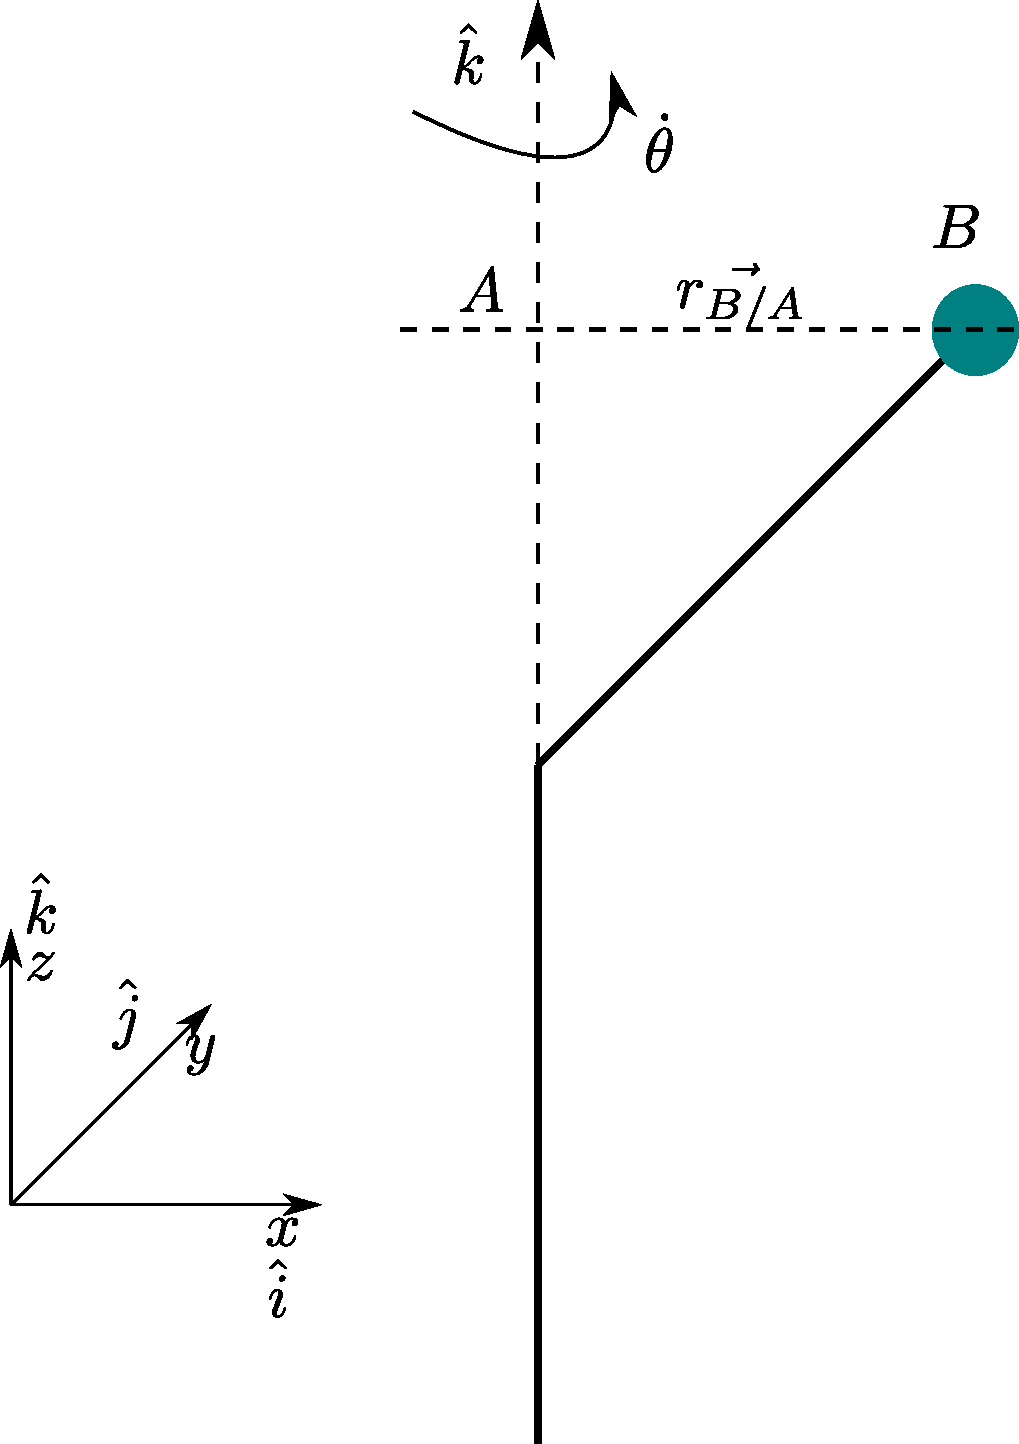
\includegraphics[width=0.5\linewidth]{Bilder/051_vel_acc_polar_coordinates.pdf}
	\caption{Problem 2 on Torque and Angular Momentum}
	\label{fig_0_ch_2_Problem2}
\end{figure}
This is a case when the velocity $v_{A/O} = 0$ in equation \eqref{eq_0_ch_0_TorqueOfAprticleEq6}, therefore, using equation \eqref{eq_0_ch_0_TorqueOfAprticleEq7}
\begin{equation}
	\tau_{B/A} = \frac{d}{dt} h_{B/A} = \frac{d}{dt} \left( m r^{2} \dot{\theta} \hat{k} \right) = 2 m r \dot{r} \dot{\theta} \hat{k} + m r^{2}\ddot{\theta} \hat{k}
\end{equation}
again as $\dot{r} = 0$, the above equation reduces to
\begin{equation}
	\tau_{B/A} = m r^{2}\ddot{\theta} \hat{k}
\end{equation}
writing the above torque equation in the form $\tau = r \times F$
\begin{equation}
	\tau_{B/A} = r_{B/A} \times F = r \hat{r} \times \left( m r^{2}\ddot{\theta} \hat{\theta} \right)
\end{equation}
therefore, the above force comes from the Euler's acceleration acting in the direction of $\hat{\theta}$.

Consider now another case, where the reference axis for calculating the distance is chosen as shown in figure \ref{fig_0_ch_2_Problem2_case2}
\newpage
\begin{figure}[h!]
	\centering
	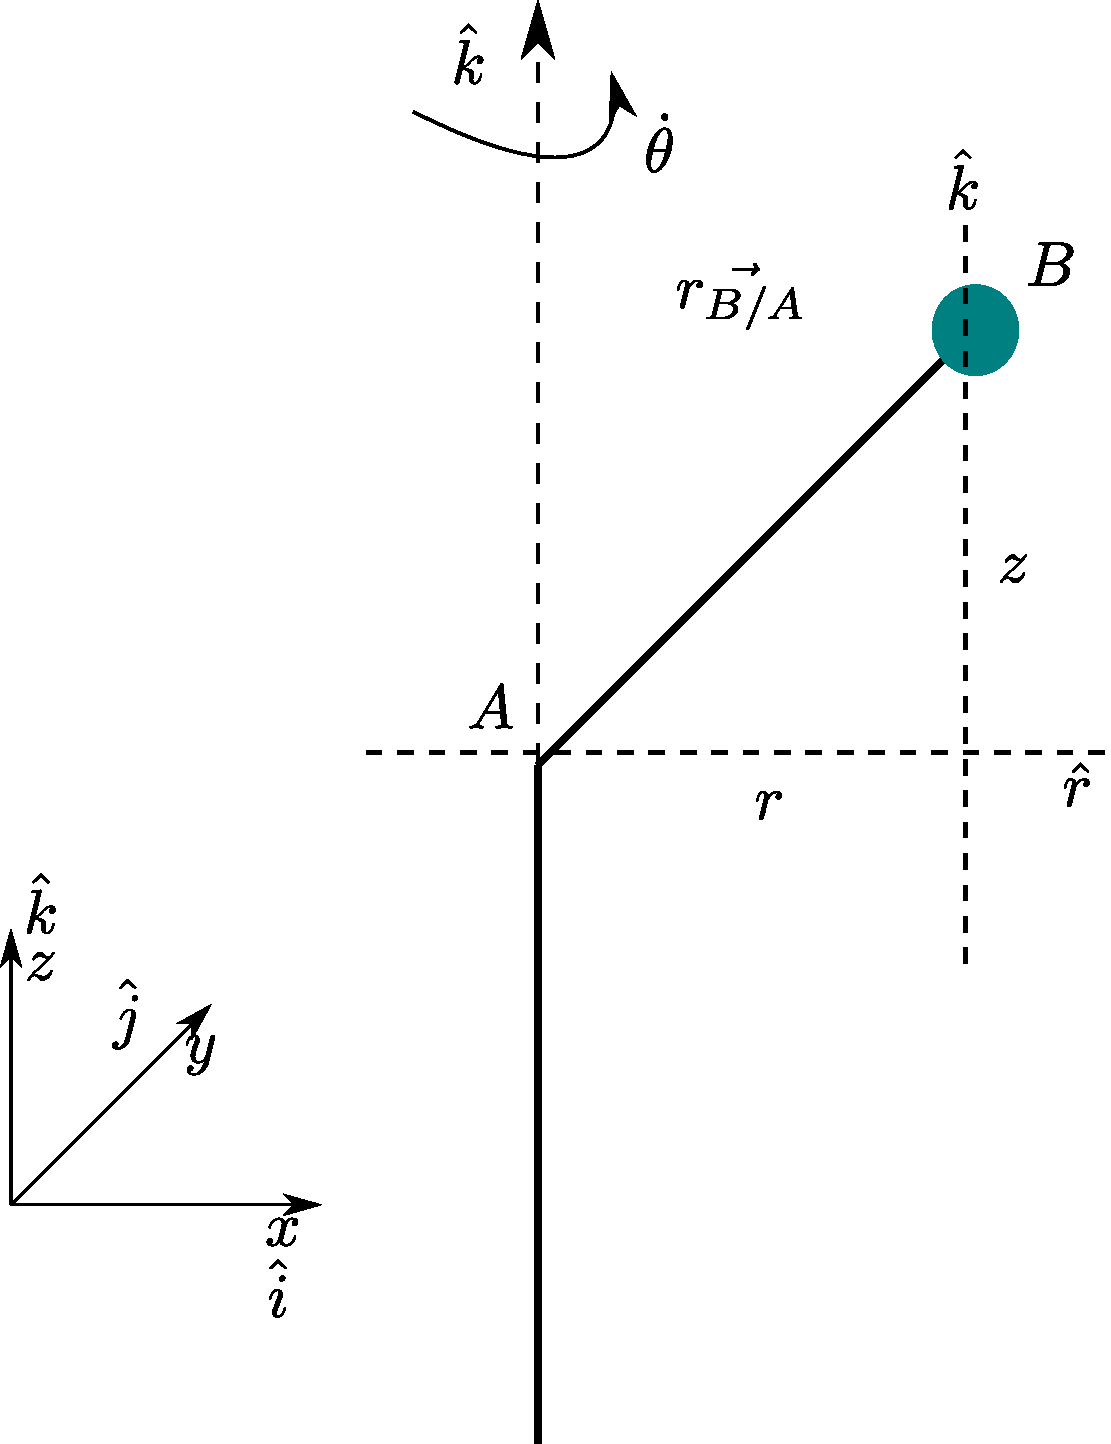
\includegraphics[width=0.5\linewidth]{Bilder/052_vel_acc_polar_coordinates.pdf}
		\caption{Problem 2 on Torque and Angular Momentum, case 2}
	\label{fig_0_ch_2_Problem2_case2}
\end{figure}
in this case now the vector $r_{B/A} = r \hat{r} + z \hat{k}$. Staring from velocity of B
\begin{equation}
v_{B/O} = v_{B/A} + \omega \times r_{B/A} = \frac{d}{dt}\left( r \hat{r} + z \hat{k} \right) + \dot{\theta} \hat{k} \times \left( r \hat{r} + z \hat{k} \right) = r \dot{\theta} \hat{\theta}
\end{equation}
linear momentum is now given by
\begin{equation}
	p_{B/O} = m v_{B/O} = m r \dot{\theta} \hat{\theta}
\end{equation}
further angular momentum is now expressed as
\begin{equation}
	h_{B/A} = r_{B/A} \times p_{B/O} =  \left(r \hat{r} + z \hat{k} \right) \times \left( m r \dot{\theta} \hat{\theta} \right)
\end{equation}
simplifying the above equation, we get
\begin{equation}
	h_{B/A} = m r^{2} \dot{\theta} \hat{k} - m r z \dot{\theta} \hat{r}
\end{equation}
again using equation \eqref{eq_0_ch_0_TorqueOfAprticleEq7} as in the earlier case
\begin{equation}
\tau_{B/A} = \frac{d}{dt} h_{B/A} = \frac{d}{dt} \left( m r^{2} \dot{\theta} \hat{k} - m r z \dot{\theta} \hat{r} \right)
\end{equation}
simplifying the above equation
\begin{equation}
	\tau_{B/A} = 2 m r \dot{r} \dot{\theta} \hat{k} + m r^{2} \ddot{\theta} \hat{k} - m r \dot{z} \dot{\theta} \hat{r} - m \dot{r} z \dot{\theta} \hat{r} - m r z \ddot{\theta} \hat{r} - m r z \dot{\theta} \dot{\hat{r}}
\end{equation}
again $\dot{r} = \dot{z} = 0$ in the above expression, therefore,
\begin{equation}
	\tau_{B/A} = m r^{2} \ddot{\theta} \hat{k} - m r z \ddot{\theta} \hat{r} - m r z \dot{\theta} \dot{\hat{r}}
\end{equation}
where $\dot{\hat{r}} = \theta \hat{\theta}$, therefore, the above equation is now expressed as
\begin{equation}
\tau_{B/A} = m r^{2} \ddot{\theta} \hat{k} - m r z \ddot{\theta} \hat{r} - m r z \dot{\theta}^2 \hat{\theta}
\end{equation}
writing the above torque equation in the form $\tau = r \times F$
\begin{equation}
\tau_{B/A} = r_{B/A} \times F = \left(r \hat{r} + z \hat{k} \right) \times \left( m r \ddot{\theta} \hat{\theta} - m r \ddot{\theta} \hat{\theta} - m r \dot{\theta}^{2} \hat{\theta} \right)
\end{equation}
therefore, from the above equation, the following forces can be defined
\begin{enumerate}
	\item $m r \ddot{\theta} \hat{\theta}$ Eulerian Acceleration
	\item $m r \ddot{\theta} \hat{\theta}$ Force applied by the mechanical link for structural stability (bending moment on the direction parallel to $\hat{\theta}$)
	\item $m r \dot{\theta}^{2} \hat{\theta}$ again this is the force applied by the mechanical link for structural stability (bending moment on the direction parallel to $\hat{r}$)
\end{enumerate}

\textbf{\textit{Note: }}From this case of dynamics problem, it can be shown therefore, that angular momentum equations can not only be used to determine the dynamics of the system, but also its static behavior, provided that the axis of reference are chosen appropriately for the kind of static information to be determined. This depends on the axis and the coordinates to be chosen in a way that the problem solution is forced to find all the acting forces onto the system.

\section{Exercise Problem}

Consider the figure \ref{Fig_0_ch_2_ExerciseProblem}. A mass $m$ is placed on a plate which can be tilted by an angle $\theta$. The angular velocity of the plate is constant $\omega = 3 rad/s$. The block of mass $m$ slips when $\theta = 50 \circ$. Derive EOM's for this problem.
\begin{figure}[h!]
	\centering
	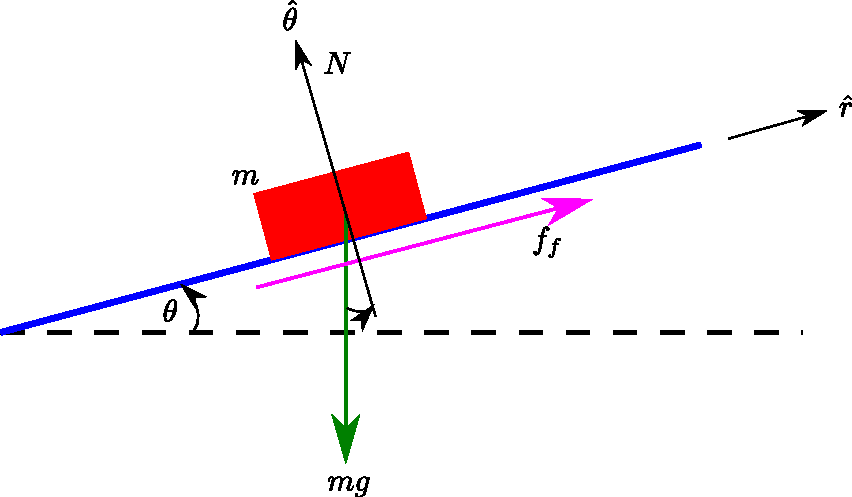
\includegraphics[width=0.65\linewidth]{Bilder/15_ExcersiceProblem.pdf}
	\caption{Exercise Problem on Inclined plane and polar coordinates}
	\label{Fig_0_ch_2_ExerciseProblem}
\end{figure}

\subsection{Chose coordinates}

Because this problem has 1D rotation, polar coordinates can reduce the complexity of the problem. The length along which the block translates if chosen along direction $\hat{r}$ and for $\hat{\theta}$ along the angular displacement of the plate. There is only one coordinate for the whole of the system (block + plate), where translating mass has coordinate $\hat{r}$, rotating plate has coordinate $\hat{\theta}$ and th whole system is constrained along $z$ direction.

\subsection{DOF}

Among the three coordinates from the polar coordinates $\hat{r}$, $\hat{\theta}$ and $\hat{k}$, translation along $\hat{k}$ is constrained, therefore, the system only has 2 DOF. For each of these 2 DOF's EOM can be derived for $\hat{r}$ and $\hat{\theta}$.

\subsection{Deriving EOM}

For the motion along $\hat{r}$ and $\hat{\theta}$, using equation \eqref{Eq_accelrationInPolarCoordinates} to find the accelerations along $\hat{r}$
\begin{equation}
a_{B/O} = a_{A/O} + (\ddot{r}\hat{r} + \ddot{z}\hat{k}) + 2 \dot{r} \dot{\theta} \hat{\theta} +  r \ddot{\theta} \hat{\theta} - r \dot{\theta}^{2} \hat{r}
\end{equation}
in this equation the terms with $\ddot{z}$ and $\ddot{\theta}$ are zero, therefore, reducing the above equation to:
\begin{equation}
a_{B/O} = a_{A/O} + \ddot{r}\hat{r} + 2 \dot{r} \dot{\theta} \hat{\theta}  - r \dot{\theta}^{2} \hat{r}
\end{equation}
further point $A$ the pivot point of the plate is also fixed, therefore the equation is reduced to
\begin{equation}
a_{B/O} = \ddot{r}\hat{r} + 2 \dot{r} \dot{\theta} \hat{\theta}  - r \dot{\theta}^{2} \hat{r}
\end{equation}

using Newtons second law, the forces along $\hat{r}$ can be expressed as
\begin{equation}\label{eq_0_ch_2_exerciseProblem1}
	\sum F_{\hat{r}} = m a_{B/O} \cdot \hat{r} = m \left[ \ddot{r}- r \dot{\theta}^{2} \right] \hat{r} 
\end{equation}
the forces along $\hat{\theta}$ can be expressed as
\begin{equation}
	\sum F_{\hat{\theta}} = m a_{B/O} \cdot \hat{\theta}  = 2 m \dot{r} \dot{\theta} \hat{\theta}
\end{equation}
in order to determine the external forces on the system along $\hat{r}$ direction, using figure \ref{Fig_0_ch_2_ExerciseProblem},
\begin{equation} \label{eq_0_ch_2_exerciseProblem}
	\sum F_{\hat{r}} = -mg sin\theta \hat{r} - f_{f} = -mg sin\theta \hat{r} + \mu mg cos\theta \hat{r}
\end{equation}
where $f_{f}$ si the frictional force acting in the direction opposite to the motion and is equal to the product of normal force $N$ and the co-efficient of friction $\mu$.

Using the same analogy, along $\hat{\theta}$ direction,
\begin{equation}
	\sum F_{\hat{\theta}} = 0
\end{equation}
because there are no external torque applied to the system. Using equation \eqref{eq_0_ch_2_exerciseProblem} with equation \eqref{eq_0_ch_2_exerciseProblem1}, the EOM along $\hat{r}$ and $\hat{\theta}$ can be expressed as
\begin{equation}
	\left[   -mg sin\theta + \mu mg cos\theta \right] \hat{r} = m \left[ \ddot{r}- r \dot{\theta}^{2} \right] \hat{r} 
\end{equation}

using this above equation of motion, any quantity can be solved for in the equation, given there is enough information about the rest of the other quantities.

For EOM along $\hat{\theta}$, the EOM is simply
\begin{equation}
\sum F_{\hat{\theta}} = 2 m \dot{r} \dot{\theta} \hat{\theta} = 0
\end{equation}
this is true as in general, when a torque is applied to the system, the Coriolis force will accelerate the block along $\dot{r}$. Because this torque is zero, the block cannot be accelerated, it can also be shown that angular momentum is conserved (which is zero in this case, i guess) as Coriolis force is zero.













